\section{536 --- Construct Binary Tree from String}
You need to construct a binary tree from a string consisting of parenthesis and integers.

The whole input represents a binary tree. It contains an integer followed by zero, one or two pairs of parenthesis. The integer represents the root's value and a pair of parenthesis contains a child binary tree with the same structure.

You always start to construct the \textbf{left} child node of the parent first if it exists.

\paragraph{Example:}

\begin{flushleft}
\textbf{Input}: $4(2(3)(1))(6(5))$

\textbf{Output}: return the tree root node representing the following tree:

\begin{figure}[H]
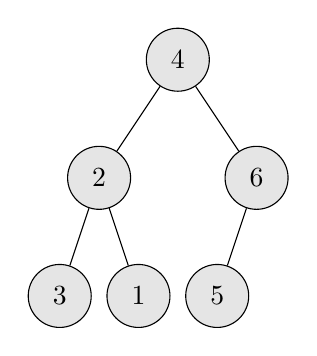
\begin{tikzpicture}
[every node/.style={draw, circle, minimum size=8mm, fill=gray!20},
level 1/.style={sibling distance=20mm},
level 2/.style={sibling distance=10mm}]
\node{4}
 child{ node{2} child {node{3}} child {node{1}}}
 child{ node{6} child {node{5}} child[missing]};
\end{tikzpicture}
\end{figure}


%       4
%     /   \
%    2     6
%   / \   / 
%  3   1 5   

\end{flushleft}

\paragraph{Note:}

\begin{itemize}
\item  There will only be parenthesis, dash and digits in the input string.
\item An empty tree is represented by empty string instead of $()$.
\end{itemize}
